\begin{question}[ID=1.1, subtitle={Discontinuità da grafico — serie 1}, tags={continuità, discontinuità, grafico}, difficulty=facile]
Determina se esistono punti di discontinuità nei grafici seguenti e indicane la tipologia.
\newline

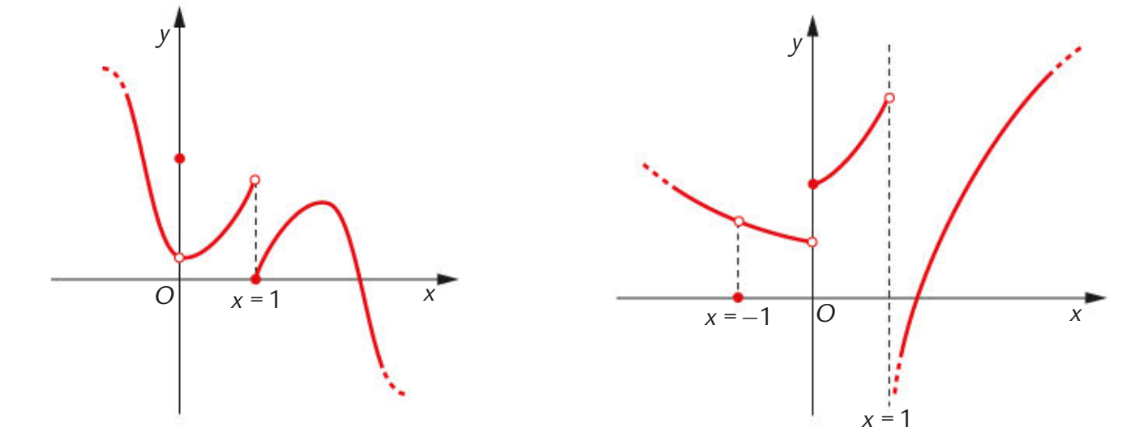
\includegraphics[width=0.9\textwidth]{images/grafici_continuità}
\begin{center}
  fig. 1 \hspace{200pt} fig. 2
\end{center}
\begin{solution}
Si legge ciascun grafico nel punto critico confrontando limite sinistro, limite destro e valore della funzione. Le tipologie sono:
\begin{itemize}
\item \textbf{eliminabile} (3ª specie): $\lim_{x\to x_0^-}f=\lim_{x\to x_0^+}f$ finiti e uguali, ma il valore manca o è diverso (buco o punto isolato);
\item \textbf{salto} (1ª specie): limite sinistro e destro finiti ma \emph{diversi}; l'ampiezza del salto è la loro differenza;
\item \textbf{2ª specie}: almeno uno dei due limiti è infinito o non esiste (tipico degli asintoti verticali).
\end{itemize}
Per ogni figura si individua il punto $x_0$ in cui il tratto si interrompe e si classifica secondo lo schema precedente.
\end{solution}
\end{question}

%---------------------------------------------------%

\begin{question}[ID=1.2, subtitle={Discontinuità da grafico — serie 2}, tags={continuità, discontinuità, grafico}, difficulty=facile]
Determina se esistono punti di discontinuità nei grafici seguenti e indicane la tipologia.
\newline

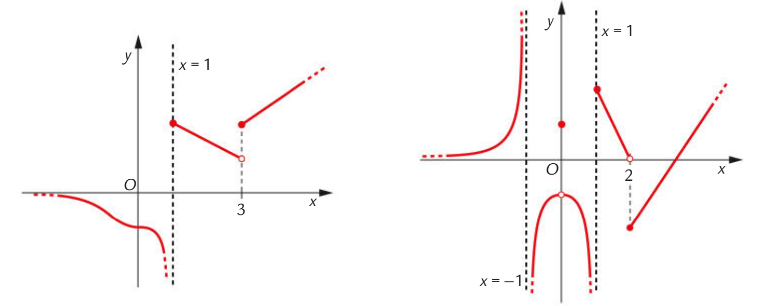
\includegraphics[width=0.9\textwidth]{images/grafici_continuità_2}
\begin{center}
  fig. 1 \hspace{200pt} fig. 2
\end{center}
\begin{solution}
Stesso metodo: nel punto in cui il grafico si interrompe si confrontano $\lim_{x\to x_0^-}f$, $\lim_{x\to x_0^+}f$ e $f(x_0)$.
\begin{itemize}
\item Limiti uguali e finiti, valore mancante o diverso $\Rightarrow$ \textbf{eliminabile};
\item limiti finiti ma diversi $\Rightarrow$ \textbf{salto} (1ª specie), di ampiezza pari alla differenza;
\item un limite infinito o inesistente $\Rightarrow$ \textbf{2ª specie} (asintoto verticale o oscillazione).
\end{itemize}
Si applica a ciascuna figura nel rispettivo punto di discontinuità.
\end{solution}
\end{question}

%---------------------------------------------------%

\begin{question}[ID=2.1, subtitle={Punti singolari — serie 1}, tags={continuità, punti singolari}, difficulty=media]
Individua e classifica gli eventuali punti singolari delle seguenti funzioni:
\begin{center}\begin{minipage}{0.92\linewidth}
\begin{multicols}{2}
\begin{enumerate}[label=\arabic*),leftmargin=3.2cm]
\item $f(x) = \frac{x^2-4}{x+2}$
\item $f(x) = \frac{\sqrt{x+2}-2}{x-2}$
\item $f(x) = \frac{|x|}{x}$
\item $f(x) = \frac{(x-2)^2}{|x-2|}$
\item $f(x) = \frac{1}{e^x-1}$
\item $f(x) = \frac{1}{1-\cos x}$
\item $f(x) = \begin{cases} x - 2 \quad & x \ge 2 \\ \frac{2x-4}{x-3} \quad & x < 2 \end{cases}$
\item $f(x) = \begin{cases} \frac{\sin x}{x} \qquad x < 0 \\ e^{1/\ln x} \qquad x > 0 \end{cases}$
\end{enumerate}
\end{multicols}
\end{minipage}\end{center}
\begin{solution}
1) $\dfrac{x^2-4}{x+2}=x-2$ per $x\neq-2$: \textbf{eliminabile} in $x=-2$ (limite $-4$). \\
2) Razionalizzando, $\dfrac{\sqrt{x+2}-2}{x-2}=\dfrac{1}{\sqrt{x+2}+2}$: \textbf{eliminabile} in $x=2$ (limite $\tfrac14$). \\
3) $\dfrac{|x|}{x}$ vale $+1$ a destra e $-1$ a sinistra: \textbf{salto} (1ª specie) in $x=0$, ampiezza $2$. \\
4) $\dfrac{(x-2)^2}{|x-2|}=|x-2|$ per $x\neq2$: \textbf{eliminabile} in $x=2$ (limite $0$). \\
5) $e^x-1=0$ in $x=0$, con limiti $\pm\infty$: \textbf{2ª specie} (asintoto verticale) in $x=0$. \\
6) $1-\cos x=0$ in $x=2k\pi$, denominatore $\to0^+$: \textbf{2ª specie} (poli) in $x=2k\pi$. \\
7) In $x=2$ entrambi i rami valgono $0$ ($\lim_{x\to2^-}\tfrac{2x-4}{x-3}=0=f(2)$): \textbf{continua}, nessun punto singolare. \\
8) In $x=0$ i due rami tendono a $1$ (buco): \textbf{eliminabile}; in $x=1$ è $\ln x\to0$ con $e^{1/\ln x}\to+\infty$ a destra: \textbf{2ª specie}.
\end{solution}
\end{question}

%---------------------------------------------------%

\begin{question}[ID=2.2, subtitle={Punti singolari — serie 2}, tags={continuità, punti singolari}, difficulty=media]
Individua e classifica gli eventuali punti singolari delle seguenti funzioni:
\begin{center}\begin{minipage}{0.92\linewidth}
\begin{multicols}{2}
\begin{enumerate}[label=\arabic*),leftmargin=3.2cm]
\item $f(x) = \frac{x^2 + 1}{x - 1}$
\item $f(x) = \frac{\ln(x+1)}{x}$
\item $f(x) = \frac{|x-1|}{x-1}$
\item $f(x) = \frac{x^3}{|x|}$
\item $f(x) = \frac{1}{\sin x}$
\item $f(x) = \frac{1}{1-\tan x}$
\item $f(x) = \begin{cases} \sqrt{x} \quad & x \ge 0 \\ x^2 \quad & x < 0 \end{cases}$
\item $f(x) = \begin{cases} e^x \qquad x \ge 0 \\ \frac{1}{x^2+1} \qquad x < 0 \end{cases}$
\end{enumerate}
\end{multicols}
\end{minipage}\end{center}
\begin{solution}
1) $\dfrac{x^2+1}{x-1}$: in $x=1$ numeratore $=2\neq0$, denominatore $\to0$: \textbf{2ª specie} (asintoto verticale). \\
2) $\dfrac{\ln(x+1)}{x}\to1$ per $x\to0$ (limite notevole): \textbf{eliminabile} in $x=0$. \\
3) $\dfrac{|x-1|}{x-1}=\pm1$: \textbf{salto} (1ª specie) in $x=1$, ampiezza $2$. \\
4) $\dfrac{x^3}{|x|}=x^2\,\mathrm{sgn}(x)\to0$: \textbf{eliminabile} in $x=0$. \\
5) $\sin x=0$ in $x=k\pi$: \textbf{2ª specie} (poli). \\
6) $\tan x=1$ in $x=\tfrac{\pi}{4}+k\pi$: \textbf{2ª specie}; nei punti $x=\tfrac{\pi}{2}+k\pi$ (dove $\tan x\to\infty$) si ha $f\to0$: \textbf{eliminabile}. \\
7) In $x=0$: $\sqrt0=0$ e $\lim_{x\to0^-}x^2=0$: \textbf{continua}. \\
8) In $x=0$: $e^0=1$ e $\lim_{x\to0^-}\tfrac{1}{x^2+1}=1$: \textbf{continua}. Nessun punto singolare.
\end{solution}
\end{question}

\begin{question}[ID=2.3, subtitle={Punti singolari — serie 3}, tags={continuità, punti singolari}, difficulty=media]
Individua e classifica gli eventuali punti singolari delle seguenti funzioni:
\begin{center}\begin{minipage}{0.92\linewidth}
\begin{multicols}{2}
\begin{enumerate}[label=\arabic*),leftmargin=3.2cm]
\item $f(x) = \frac{x^2 - x}{x^2 + x}$
\item $f(x) = \frac{\sqrt{x}}{x-1}$
\item $f(x) = \frac{|x+3|}{x+3}$
\item $f(x) = \frac{x^2 - 4x}{|x-2|}$
\item $f(x) = \frac{1}{e^{x^2}-1}$
\item $f(x) = \frac{1}{\cos x - 1}$
\item $f(x) = \begin{cases} x^3 - 1 \quad & x > 1 \\ \frac{x}{x+1} \quad & x \le 1 \end{cases}$
\item $f(x) = \begin{cases} \ln(x) \qquad x > 1 \\ x^2 - 2x + 1 \qquad x \le 1 \end{cases}$
\end{enumerate}
\end{multicols}
\end{minipage}\end{center}
\begin{solution}
1) $\dfrac{x^2-x}{x^2+x}=\dfrac{x-1}{x+1}$ per $x\neq0$: \textbf{eliminabile} in $x=0$ (limite $-1$), \textbf{2ª specie} in $x=-1$. \\
2) $\dfrac{\sqrt{x}}{x-1}$ (dominio $x\ge0$): in $x=1$ numeratore $=1\neq0$: \textbf{2ª specie}. \\
3) $\dfrac{|x+3|}{x+3}=\pm1$: \textbf{salto} (1ª specie) in $x=-3$, ampiezza $2$. \\
4) $\dfrac{x^2-4x}{|x-2|}$: in $x=2$ numeratore $=-4\neq0$, $f\to-\infty$: \textbf{2ª specie}. \\
5) $e^{x^2}-1=0$ solo in $x=0$, $f\to+\infty$: \textbf{2ª specie}. \\
6) $\cos x=1$ in $x=2k\pi$, $f\to-\infty$: \textbf{2ª specie}. \\
7) In $x=1$: $\lim_{x\to1^+}(x^3-1)=0$ ma $f(1)=\tfrac{1}{2}$: \textbf{salto} (1ª specie), ampiezza $\tfrac12$; inoltre \textbf{2ª specie} in $x=-1$ (dove $\tfrac{x}{x+1}$ esplode). \\
8) In $x=1$: $\lim_{x\to1^+}\ln x=0=(1-1)^2$: \textbf{continua}.
\end{solution}
\end{question}

%---------------------------------------------------%

\begin{question}[ID=2.4, subtitle={Punti singolari — serie 4}, tags={continuità, punti singolari}, difficulty=media]
Individua e classifica gli eventuali punti singolari delle seguenti funzioni:
\begin{center}\begin{minipage}{0.92\linewidth}
\begin{multicols}{2}
\begin{enumerate}[label=\arabic*),leftmargin=3.2cm]
\item $f(x) = \frac{x^3 - 3x}{x^2 - 1}$
\item $f(x) = \frac{\sqrt{x+1}}{x+2}$
\item $f(x) = \frac{|x|}{x^2}$
\item $f(x) = \frac{(x-3)^2}{|x-3|}$
\item $f(x) = \frac{1}{e^{x+1} - 2}$
\item $f(x) = \frac{1}{\tan x}$
\item $f(x) = \begin{cases} x^2 - 1 \quad & x \neq 0 \\ 1 \quad & x = 0 \end{cases}$
\item $f(x) = \begin{cases} \sin x \qquad x > 0 \\ x - 2 \qquad x \le 0 \end{cases}$
\end{enumerate}
\end{multicols}
\end{minipage}\end{center}
\begin{solution}
1) $\dfrac{x^3-3x}{x^2-1}$: in $x=\pm1$ numeratore $\neq0$: \textbf{2ª specie} in $x=1$ e $x=-1$. \\
2) $\dfrac{\sqrt{x+1}}{x+2}$ (dominio $x\ge-1$): $x=-2$ è fuori dal dominio, quindi \textbf{nessun punto singolare}. \\
3) $\dfrac{|x|}{x^2}=\dfrac{1}{|x|}\to+\infty$: \textbf{2ª specie} in $x=0$. \\
4) $\dfrac{(x-3)^2}{|x-3|}=|x-3|$: \textbf{eliminabile} in $x=3$ (limite $0$). \\
5) $e^{x+1}-2=0$ in $x=\ln2-1$: \textbf{2ª specie}. \\
6) $\dfrac{1}{\tan x}$: $\tan x=0$ in $x=k\pi$ $\Rightarrow$ \textbf{2ª specie}; in $x=\tfrac{\pi}{2}+k\pi$ vale $0$: \textbf{eliminabile}. \\
7) In $x=0$: $\lim(x^2-1)=-1$ ma $f(0)=1$: \textbf{eliminabile} (limite finito $\neq$ valore). \\
8) In $x=0$: $\lim_{x\to0^+}\sin x=0$ ma $f(0)=-2$: \textbf{salto} (1ª specie), ampiezza $2$.
\end{solution}
\end{question}

%---------------------------------------------------%

\begin{question}[ID=2.5, subtitle={Punti singolari — serie 5}, tags={continuità, punti singolari}, difficulty=media]
Individua e classifica gli eventuali punti singolari delle seguenti funzioni:
\begin{center}\begin{minipage}{0.92\linewidth}
\begin{multicols}{2}
\begin{enumerate}[label=\arabic*),leftmargin=3.2cm]
\item $f(x) = \frac{x^2 + 4x + 4}{x^2 - 4}$
\item $f(x) = \frac{\sqrt{x^2 - 1}}{x-1}$
\item $f(x) = \frac{|x-1|}{x^2 - 1}$
\item $f(x) = \frac{x+2}{|x+2|}$
\item $f(x) = \frac{1}{e^x+1}$
\item $f(x) = \frac{1}{\sin x - x}$
\item $f(x) = \begin{cases} x^2 \quad & x \geq 2 \\ 2x - 1 \quad & x < 2 \end{cases}$
\item $f(x) = \begin{cases} e^{-x} \qquad x > 0 \\ x + 3 \qquad x \le 0 \end{cases}$
\end{enumerate}
\end{multicols}
\end{minipage}\end{center}
\begin{solution}
1) $\dfrac{x^2+4x+4}{x^2-4}=\dfrac{x+2}{x-2}$ per $x\neq-2$: \textbf{eliminabile} in $x=-2$ (limite $0$), \textbf{2ª specie} in $x=2$. \\
2) $\dfrac{\sqrt{x^2-1}}{x-1}$ (dominio $x\le-1$ o $x\ge1$): in $x=1$ il limite destro è $+\infty$: \textbf{2ª specie}. \\
3) $\dfrac{|x-1|}{x^2-1}=\dfrac{|x-1|}{(x-1)(x+1)}$: \textbf{salto} in $x=1$ (limiti $\pm\tfrac12$, ampiezza $1$), \textbf{2ª specie} in $x=-1$. \\
4) $\dfrac{x+2}{|x+2|}=\pm1$: \textbf{salto} (1ª specie) in $x=-2$, ampiezza $2$. \\
5) $e^x+1>0$ sempre: \textbf{nessun punto singolare}. \\
6) $\sin x-x=0$ solo in $x=0$, con $f\to-\infty$: \textbf{2ª specie} in $x=0$. \\
7) In $x=2$: $f(2)=4$ ma $\lim_{x\to2^-}(2x-1)=3$: \textbf{salto} (1ª specie), ampiezza $1$. \\
8) In $x=0$: $\lim_{x\to0^+}e^{-x}=1$ ma $f(0)=3$: \textbf{salto} (1ª specie), ampiezza $2$.
\end{solution}
\end{question}

%---------------------------------------------------%

\begin{question}[ID=2.6, subtitle={Punti singolari — serie 6}, tags={continuità, punti singolari}, difficulty=media]
Individua e classifica gli eventuali punti singolari delle seguenti funzioni:
\begin{center}\begin{minipage}{0.92\linewidth}
\begin{multicols}{2}
\begin{enumerate}[label=\arabic*),leftmargin=3.2cm]
\item $f(x) = \frac{2x+1}{x^2-x}$
\item $f(x) = \frac{\ln(x^2+1)}{x-1}$
\item $f(x) = \frac{|x+1|}{x-1}$
\item $f(x) = \frac{(x-1)^3}{|x+1|}$
\item $f(x) = \frac{1}{e^{x-1} - 1}$
\item $f(x) = \frac{1}{\cos(x)-1}$
\item $f(x) = \begin{cases} x^3 - 1 \quad & x > 0 \\ x^2 - 2x \quad & x \le 0 \end{cases}$
\item $f(x) = \begin{cases} \tan x \qquad x > 0 \\ x^3 - x \qquad x \le 0 \end{cases}$
\end{enumerate}
\end{multicols}
\end{minipage}\end{center}
\begin{solution}
1) $\dfrac{2x+1}{x^2-x}=\dfrac{2x+1}{x(x-1)}$: \textbf{2ª specie} in $x=0$ e $x=1$. \\
2) $\dfrac{\ln(x^2+1)}{x-1}$: in $x=1$ numeratore $=\ln2\neq0$: \textbf{2ª specie}. \\
3) $\dfrac{|x+1|}{x-1}$: in $x=1$ numeratore $=2\neq0$: \textbf{2ª specie} (in $x=-1$ vale $0$, continua). \\
4) $\dfrac{(x-1)^3}{|x+1|}$: in $x=-1$ numeratore $=-8\neq0$: \textbf{2ª specie}. \\
5) $e^{x-1}-1=0$ in $x=1$: \textbf{2ª specie}. \\
6) $\cos x=1$ in $x=2k\pi$: \textbf{2ª specie}. \\
7) In $x=0$: $\lim_{x\to0^+}(x^3-1)=-1$ ma $f(0)=0$: \textbf{salto} (1ª specie), ampiezza $1$. \\
8) In $x=0$: $\lim_{x\to0^+}\tan x=0=f(0)$: \textbf{continua}; restano \textbf{2ª specie} nei poli $x=\tfrac{\pi}{2}+k\pi$ ($k\ge0$).
\end{solution}
\end{question}

%---------------------------------------------------%

\begin{question}[ID=3.1, subtitle={Teorema degli zeri per $e^x-2x^2$ su $[0,2]$}, tags={continuità, teorema degli zeri}, difficulty=media]
Stabilisci se la funzione soddisfa le ipotesi del \textit{teorema di esistenza degli zeri} nell'intervallo indicato, motivando adeguatamente la risposta e, se soddisfatte, trovane gli zeri.
\begin{center}
    $f(x) = e^x - 2x^2$ \qquad $[0,2]$
\end{center}
\begin{solution}
$f$ continua su $[0,2]$; $f(0)=1>0$, $f(2)=e^2-8<0$: esiste uno zero in $(0,2)$.
\end{solution}
\end{question}

%---------------------------------------------------%

\begin{question}[ID=3.2, subtitle={Teorema degli zeri per $\sin x - x/2$ su $[0,\pi]$}, tags={continuità, teorema degli zeri}, difficulty=facile]
Verifica se la funzione soddisfa le ipotesi del \textit{teorema di esistenza degli zeri} nell'intervallo indicato. Se le ipotesi sono soddisfatte, determina almeno uno zero della funzione.
\begin{center}
    $f(x) = \sin(x) - \dfrac{x}{2}$ \qquad $[0, \pi]$
\end{center}
\begin{solution}
$f(0)=0$: $x=0$ è già uno zero. $f(\pi)=-\pi/2<0$; esiste anche uno zero in $(0,\pi)$.
\end{solution}
\end{question}

%---------------------------------------------------%

\begin{question}[ID=3.3, subtitle={Teorema degli zeri per $\ln x + x - 3$ su $[1,4]$}, tags={continuità, teorema degli zeri}, difficulty=media]
Stabilisci se la funzione data soddisfa le condizioni richieste dal \textit{teorema di esistenza degli zeri} nell'intervallo specificato. Spiega il ragionamento e, se possibile, calcola uno zero.
\begin{center}
    $f(x) = \ln(x) + x - 3$ \qquad $[1, 4]$
\end{center}
\begin{solution}
$f(1)=-2<0$, $f(4)=\ln4+1>0$: esiste uno zero in $(1,4)$.
\end{solution}
\end{question}

%---------------------------------------------------%

\begin{question}[ID=3.4, subtitle={Teorema degli zeri per $x^3-3x+1$ su $[-2,1]$}, tags={continuità, teorema degli zeri}, difficulty=media]
Analizza la funzione nell'intervallo indicato per verificare l'applicabilità del \textit{teorema di esistenza degli zeri}. Se il teorema si applica, determina gli zeri (se possibile) o stima il loro valore.
\begin{center}
    $f(x) = x^3 - 3x + 1$ \qquad $[-2, 1]$
\end{center}
\begin{solution}
$f(-2)=-1<0$, $f(0)=1>0$, $f(1)=-1<0$: esistono due zeri, in $(-2,0)$ e in $(0,1)$.
\end{solution}
\end{question}

%---------------------------------------------------%

\begin{question}[ID=3.5, subtitle={Teorema degli zeri per $e^{-x}-\cos x$ su $[0,\pi/2]$}, tags={continuità, teorema degli zeri}, difficulty=media]
Dimostra se il \textit{teorema di esistenza degli zeri} è applicabile alla funzione considerata nell'intervallo specificato. Nel caso affermativo, calcola o stima almeno uno zero.
\begin{center}
    $f(x) = e^{-x} - \cos(x)$ \qquad $[0, \pi/2]$
\end{center}
\begin{solution}
$f(0)=0$: $x=0$ è già uno zero della funzione.
\end{solution}
\end{question}

%---------------------------------------------------%

\begin{question}[ID=4.1, subtitle={Continuità e salto di $f$ con $e^x-k$ e $x^3+k$ in $x=0$}, tags={continuità, parametrico}, difficulty=media]
Determina per quali valori di $k$ la funzione
\[
f(x) = \begin{cases}
    e^x - k \qquad x < 0 \\
    x^3+k \qquad x \ge 0
\end{cases}
\]
\begin{enumerate}
\item è continua in $x=0$
\item presenti un punto di salto in $x=0$, con salto uguale a $2$
\end{enumerate}
\begin{solution}
1) $1-k=k \Rightarrow k=\tfrac{1}{2}$. 2) $|1-2k|=2 \Rightarrow k=-\tfrac{1}{2}$ oppure $k=\tfrac{3}{2}$.
\end{solution}
\end{question}

%---------------------------------------------------%

\begin{question}[ID=4.2, subtitle={Continuità e salto di $f$ con $\ln(1+x)-k$ e $kx^2-1$ in $x=1$}, tags={continuità, parametrico}, difficulty=media]
Determina per quali valori di $k$ la funzione
\[
f(x) = \begin{cases}
    \ln(1+x) - k \qquad x < 1 \\
    kx^2 - 1 \qquad x \ge 1
\end{cases}
\]
\begin{enumerate}
\item è continua in $x=1$
\item presenti un punto di salto in $x=1$, con salto uguale a $1$
\end{enumerate}
\begin{solution}
1) $\ln2-k=k-1 \Rightarrow k=\tfrac{\ln2+1}{2}$. 2) $|\ln2+1-2k|=1 \Rightarrow k=\tfrac{\ln2}{2}$ oppure $k=\tfrac{\ln2+2}{2}$.
\end{solution}
\end{question}

%---------------------------------------------------%

\begin{question}[ID=4.3, subtitle={Continuità e salto di $f$ con $x^2-kx$ e $kx+3$ in $x=-1$}, tags={continuità, parametrico}, difficulty=media]
Trova i valori di $k$ per cui la funzione
\[
f(x) = \begin{cases}
    x^2 - kx \qquad x < -1 \\
    kx + 3 \qquad x \ge -1
\end{cases}
\]
\begin{enumerate}
\item è continua in $x=-1$
\item presenti un punto di salto in $x=-1$, con salto uguale a $4$
\end{enumerate}
\begin{solution}
1) $1+k=-k+3 \Rightarrow k=1$. 2) $|2k-2|=4 \Rightarrow k=3$ oppure $k=-1$.
\end{solution}
\end{question}

%---------------------------------------------------%

\begin{question}[ID=4.4, subtitle={Continuità e salto di $f$ con $kx-2$ e $4x+k$ in $x=2$}, tags={continuità, parametrico}, difficulty=media]
Determina per quali valori di $k$ la funzione
\[
f(x) = \begin{cases}
    kx - 2 \qquad x < 2 \\
    4x + k \qquad x \ge 2
\end{cases}
\]
\begin{enumerate}
\item è continua in $x=2$
\item presenti un punto di salto in $x=2$, con salto uguale a $3$
\end{enumerate}
\begin{solution}
1) $2k-2=8+k \Rightarrow k=10$. 2) $|k-10|=3 \Rightarrow k=13$ oppure $k=7$.
\end{solution}
\end{question}

%---------------------------------------------------%

\begin{question}[ID=4.5, subtitle={Continuità e salto di $f$ con $k+\sin x$ e $k\cos x$ in $x=\pi/2$}, tags={continuità, parametrico}, difficulty=media]
Stabilisci i valori di $k$ per cui la funzione
\[
f(x) = \begin{cases}
    k + \sin(x) \qquad x < \dfrac{\pi}{2} \\
    k\cos(x) \qquad x \ge \dfrac{\pi}{2}
\end{cases}
\]
\begin{enumerate}
\item è continua in $x=\dfrac{\pi}{2}$
\item presenti un punto di salto in $x=\dfrac{\pi}{2}$, con salto uguale a $\dfrac{1}{2}$
\end{enumerate}
\begin{solution}
1) $k+1=0 \Rightarrow k=-1$. 2) $|k+1|=\tfrac{1}{2} \Rightarrow k=-\tfrac{1}{2}$ oppure $k=-\tfrac{3}{2}$.
\end{solution}
\end{question}

%---------------------------------------------------%

\begin{question}[ID=4.6, subtitle={Continuità e salto di $f$ con $kx^2+1$ e $e^x-k$ in $x=0$}, tags={continuità, parametrico}, difficulty=media]
Determina per quali valori di $k$ la funzione
\[
f(x) = \begin{cases}
    kx^2 + 1 \qquad x < 0 \\
    e^x - k \qquad x \ge 0
\end{cases}
\]
\begin{enumerate}
\item è continua in $x=0$
\item presenti un punto di salto in $x=0$, con salto uguale a $5$
\end{enumerate}
\begin{solution}
1) $1=1-k \Rightarrow k=0$. 2) $|k|=5 \Rightarrow k=\pm5$.
\end{solution}
\end{question}

%---------------------------------------------------%

\begin{question}[ID=5.1, subtitle={Asintoti di $f(x)=(x^2+1)/(x-1)$}, tags={continuità, asintoti}, difficulty=media]
Studia la seguente funzione ponendo particolare attenzione a eventuali asintoti:
\begin{equation*}
    f(x) =\frac{x^2+1}{x-1}
\end{equation*}
\begin{solution}
Asintoto verticale $x=1$; asintoto obliquo $y=x+1$ (divisione: $x^2+1=(x-1)(x+1)+2$).
\end{solution}
\end{question}

%---------------------------------------------------%

\begin{question}[ID=5.2, subtitle={Asintoti di $f(x)=(x^2-4)/(x+2)$}, tags={continuità, asintoti}, difficulty=facile]
Studia la seguente funzione ponendo particolare attenzione a eventuali asintoti:
\begin{equation*}
    f(x) = \frac{x^2 - 4}{x+2}
\end{equation*}
\begin{solution}
$f(x)=x-2$ per $x\ne-2$: buco (discontinuità eliminabile) in $x=-2$, nessun asintoto.
\end{solution}
\end{question}

%---------------------------------------------------%

\begin{question}[ID=5.3, subtitle={Asintoti di $f(x)=(2x+3)/(x^2-1)$}, tags={continuità, asintoti}, difficulty=media]
Analizza la seguente funzione razionale determinando la presenza di eventuali asintoti verticali, orizzontali o obliqui:
\begin{equation*}
    f(x) = \frac{2x+3}{x^2-1}
\end{equation*}
\begin{solution}
Asintoti verticali $x=1$ e $x=-1$; asintoto orizzontale $y=0$.
\end{solution}
\end{question}

%---------------------------------------------------%

\begin{question}[ID=5.4, subtitle={Asintoti di $f(x)=(x^3-2x)/(x^2+1)$}, tags={continuità, asintoti}, difficulty=media]
Studia la funzione seguente, soffermandoti su eventuali asintoti e sul comportamento per $x \to \pm\infty$:
\begin{equation*}
    f(x) = \frac{x^3 - 2x}{x^2+1}
\end{equation*}
\begin{solution}
Nessun asintoto verticale; asintoto obliquo $y=x$ (poiché $x^3-2x=(x^2+1)x-3x$, quindi $f(x)=x-\tfrac{3x}{x^2+1}\to x$).
\end{solution}
\end{question}

%---------------------------------------------------%

\begin{question}[ID=5.5, subtitle={Asintoti di $f(x)=(x^2+x+1)/(x^2-2x)$}, tags={continuità, asintoti}, difficulty=media]
Determina il dominio della funzione e analizza eventuali asintoti:
\begin{equation*}
    f(x) = \frac{x^2 + x + 1}{x^2 - 2x}
\end{equation*}
\begin{solution}
Asintoti verticali $x=0$ e $x=2$; asintoto orizzontale $y=1$.
\end{solution}
\end{question}

%---------------------------------------------------%

\begin{question}[ID=5.6, subtitle={Asintoti di $f(x)=\sqrt{x^2+1}/(x-3)$}, tags={continuità, asintoti}, difficulty=media]
Studia la funzione seguente, con particolare attenzione agli asintoti verticali e orizzontali:
\begin{equation*}
    f(x) = \frac{\sqrt{x^2+1}}{x-3}
\end{equation*}
\begin{solution}
Asintoto verticale $x=3$; asintoti orizzontali $y=1$ (per $x\to+\infty$) e $y=-1$ (per $x\to-\infty$).
\end{solution}
\end{question}
